\documentclass[11pt]{article}
\usepackage{amsmath}
%\usepackage[sc]{mathpazo} %Like Palatino with extensive math support
\usepackage{fullpage}
\usepackage[authoryear]{natbib}
\linespread{1.7}
\usepackage[utf8]{inputenc}
\usepackage{lineno}
\usepackage{titlesec}
\usepackage{xcolor}
\usepackage{graphicx}
\usepackage{placeins}
\usepackage{float}
\usepackage{subfigure}
\newcommand{\tom}[2]{{\color{red}{#1}}\footnote{\textit{\color{red}{#2}}}} 
\newcommand{\ali}[2]{{\color{blue}{#1}}\footnote{\textit{\color{blue}{#2}}}}  
\usepackage{hyperref}


\titleformat{\section}[block]{\Large\bfseries\filcenter}{\thesection}{1em}{}
\titleformat{\subsection}[block]{\Large\itshape\filcenter}{\thesubsection}{1em}{}
\titleformat{\subsubsection}[block]{\large\itshape}{\thesubsubsection}{1em}{}
\titleformat{\paragraph}[runin]{\itshape}{\theparagraph}{1em}{}[.]\renewcommand{\refname}{Literature Cited}


%%%%%%%%%%%%%%%%%%%%%
% Line numbering
%%%%%%%%%%%%%%%%%%%%%
%
% Please use line numbering with your initial submission and
% subsequent revisions. After acceptance, please turn line numbering
% off by adding percent signs to the lines %\usepackage{lineno} and
% to %\linenumbers{} and %\modulolinenumbers[3] below.
%
% To avoid line numbering being thrown off around math environments,
% the math environments have to be wrapped using
% \begin{linenomath*} and \end{linenomath*}
%
% (Thanks to Vlastimil Krivan for pointing this out to us!)

\title{Thank you, next: demographic consequences of partner diversity and turnover in a multi-species ant-plant mutualism}
% title suggestion, trying to move away from focus on IPM

\author{Alexandra Campbell$^{1,\dagger}$ \\ 
	Tom E.X. Miller$^{1,\ast}$}

\date{}

\begin{document}
	
	\maketitle
	
	\noindent{} 1. Program in Ecology and Evolutionary Biology, Department of BioSciences, Rice University, Houston, Texas 77005;
	
	\noindent{} $\dagger$ e-mail: amc49@rice.edu\\
	\noindent{} $\ast$ e-mail: tom.miller@rice.edu
	
	\bigskip
	
	\textit{Keywords}: Integral Projection Model, \textit{Cylindropuntia imbricata}, population fitness, multi-species mutualism, complementarity, sampling effect, portfolio effect
	
	\bigskip
	
	\textit{Manuscript type}: Article.
	
	\bigskip
	
	\noindent{\footnotesize Prepared using the suggested \LaTeX{} template for \textit{Am.\ Nat.}}
	
\linenumbers{}
\modulolinenumbers[3]

\newpage{}

	\section*{Abstract}
% 200 words max
Mutualisms commonly involve multiple partner species but the ecological consequences of partner diversity remain poorly understood.
Partner diversity may benefit a focal mutualist through mechanisms that mirror positive effects of species diversity on ecosystem function, such as complementarity or portfolio effect. 
We studied the fitness consequences of partner diversity and turnover in the multi-species food-for-protection mutualism involving an EFN-bearing plant (tree cholla cactus \textit{Cylindropuntia imbricata}) and multiple species of nectar-feeding ants (\textit{Crematogaster opuntiae}, \textit{Liometopum apiculatum}, and other less frequent ants) that provide defense from herbivores. 
We used long-term data and Bayesian hierarchical statistical models to determine the demographic impacts of different ant partners, and the dynamics of turnover from one exclusive partner association to another. 
We then constructed a stochastic, multi-state Integral Projection Model (IPM) with which we simulated tree cholla populations with different richness and composition of partners.
We found that, while ant partners had different impacts on plant vital rates (\textit{C. opuntiae}-tended plants had advantages in growth and survival when small, and \textit{L. apiculatum}-tended plants had floral viability advantages), plant fitness was effectively insensitive to partner identity and number, because effects on the highest-sensitivity vital rates were consistent across partner species. 
Furthermore, there was no evidence that benefits of partner diversity manifest in the context of fluctuating environments (i.e., the portfolio effect). 
In contrast to much of the previous literature, this study highlights that demographic benefits of mutualism can be surprisingly robust to diversity and turnover of partners.


\newpage{}
\section*{Introduction}
Mutualisms are species interactions where all participants receive net benefits, leading to higher individual fitness and increased population growth rates. 
They are widespread species interactions but can deteriorate into commensalism or parasitism under conditions that elevate costs or dampen benefits \citep{Rodriguez-Rodriguez2017,Song2020,Mandyam2014,Thrall2007, Bahia2022,Bronstein1994,Chamberlain2014,Frederickson2013,Axelrod1981,Leigh2010}.
Mutualisms are considered more context dependent than other species interactions \citep{Chamberlain2014,Frederickson2013}, meaning the magnitude and sign of interaction strength are often determined by environmental conditions and species' identities \citep{Noe1994,Leigh2010}.

Mutualism is defined at the level of a species pair (+/+) but these interactions are embedded within multi-species communities, and growing evidence suggests that pairwise interactions are poor predictors of the net effects of multi-species mutualism \citep{Afkhami2014,Palmer2010,Bascompte2009,Dattilo2014}. 
A focal mutualist may interact with multiple guilds of partner types (e.g., plants that interact with pollinators, seed dispersers, soil microbes, and ant defenders) or with multiple partner species within the same guild (e.g., plants visited by multiple pollinator species). 
Within a mutualist guild, partner species often differ in the amount or type of goods or services they provide, making partner identity an important source of contingency in mutualism \citep{Stanton2003}. 
Whether and how partner diversity modifies the demographic effects of mutualistic interactions remain open questions within relevance in applied settings \citep{rogers2014, Thibaut2012, Frederickson2005, Palmer2010}.

There are multiple mechanisms by which partner diversity can influence the net benefits accrued by a focal mutualist, mirroring the mechanisms by which, at a larger scale of organization, biodiversity can influence ecosystem function \tom{\citep{Barrett2015,Ushio2020}.}{Cite the Winfree chapter?} 
First, when there is a hierarchy of fitness effects (a consistent ranking of best to worst mutualists), a more diverse sample of the partner community may be more likely to include the best partner \citep{Frederickson2013}.
This can lead to an apparent benefit of diversity driven by a sampling effect \citep{Batstone2018} -- but there is no benefit of diversity \emph{per se}, only better and worse partners. 
However, if partner associations are mutually exclusive (a focal mutualist may engage with only one partner at a time), then partner diversity may impose opportunity costs, leading to negative effects of a diverse mutualist assemblage relative to exclusive association with the single best partner \citep{Miller2007}. 
Second, even within a single mutualist guild, the benefits conferred by alternative partner species can vary in type and not just degree \citep{Stachowicz2005,Bronstein2006,Stanton2003}. 
This can lead to a positive effect of partner diversity through complementarity of alternative functions \citep{Batstone2018}. 
Positive diversity effects through complementarity need not be additive: interference or synergies between partners can make their combined effect different than the expected from the sum of complementary functions \citep{Afkhami2014}. 
Third, partner species can have species-specific responses to environmental variation, either spatially \citep{Ollerton2006} or temporally \citep{Alarcon2008}. 
Multiple partners can therefore act as a 'portfolio' that stabilizes fitness benefits across spatial or temporal heterogeneity, leading to positive effects of partner diversity through the portfolio effect \citep{Batstone2018,Lazaro2022,Horvitz1990}. 

Partner diversity can have different effects on a focal mutualist depending on whether partners are present simultaneously or sequentially (partner turnover) \citep{Djieto-Lordon2005, Ness2006, Bruna2014,Barrett2015,Ushio2020,Dattilo2014}. 
Sequential associations are likely when alternative partners engage in interference competition for access to a shared mutualist \citep{Kiers2003,Batstone2018,Tgaard2015,Wulff2008}. 
Turnover can happen at different timescales, from minutes to years \citep{Oliveira1999,Horvitz1986}. 
The frequency of partner turnover can impact the level of benefits received by the focal mutualist, particularly if the benefits continue to accumulate with successive turnover (e.g., when sequential partners provide complementary functions) or if they saturate over time \citep{Sachs2004,Fiala1994}.
Directionality of turnover can also influence effects of partner diversity if partner identity changes consistently across ontogeny of a focal mutualist \citep{Fonseca2003,Noe1994,Dejean2008}.
For example, plant susceptibility to enemies can change across life stages \citep{Boege2005,Barton2010}, so the benefits of a diverse guild of defensive mutualists are greatest when more defensive partner species align with more vulnerable life stages \citep{Djieto-Lordon2005,Dejean2008}.
Thus, the duration and order of interactions may be just as important as the identities of the interacting partners.

Defensive ant-plant mutualisms -- where plants provide food and/or housing to ants that in turn defend them from enemies -- are widespread interactions that offer valuable model systems for the ecology and evolution of mutualism \citep{Bronstein1998, Bronstein2006}. 
Extrafloral nectar (EFN) -bearing plants can serve as dietary resources that promote ant abundance and colony size \citep{Byk2011, Ness2009, Ness2006, Donald2022}.
In turn, presence of defensive ant partners is often linked to reductions in herbivory  \citep{Trager2010, Rudgers2004} and demographic advantages for the plant partner \citep{Baez2016}.
Defensive ant-plant mutualisms are commonly multi-species, where a guild of ant partner species share, and often compete for, a plant mutualist \citep{Bronstein1998, Beattie1985, Trager2010, Agrawal1998}.
Ant partners can vary in their ability to deter herbivores \citep{Bruna2014}, and visitation by low quality ant partners can prevent visitation by higher quality partners, causing a reduction in fitness through missed opportunity costs \citep{Fraser2001, Frederickson2005}.
Susceptibility to herbivory can also vary significantly throughout the life stages of the plant \citep{Boege2005}, suggesting that the order and timing of successive partners is important to the fitness impacts of the combined partner guild \citep{Barton2010, Boege2005, Fonseca2003}.
Finally, herbivore identity and pressure can vary inter-annually \citep{Wetzel2023}, much like mutualist identity and presence, meaning the threat plants face can vary just as much as the protection they receive due to temporal stochasticity. 
Previous studies have investigated how ant partner diversity affects plant fitness \tom{\citep{Palmer2010,Afkhami2014,Fiala1994,Gaume1998,Dattilo2014,Ludka2015}. }{The Afkhami paper cited here is not an ant-plant study.}
However, little is known about the combined effects of partner identity, directional partner turnover, and temporal stochasticity, particularly because the long-term data needed to quantify fluctuations in ant-plant interactions are rarely available. 
	
This study examined the consequences of partner diversity in a food-for-protection mutualism between the tree cholla cactus (\textit{Cylindropuntia imbricata}), a long-lived EFN-bearing plant, and multiple species of ant partners.
Tree cholla are tended by two common ant partners and several additional rarer species, all of which collect EFN in exchange for defense against herbivores.
These ant species locally co-occur but individual plants are typically tended by only one species that patrols the plant around-the-clock and maintains control of the plant's nectar resources, usually for an entire growing season \citep{Ohm2014, Donald2022}. 
Switches between partner species, or between vacancy and ant occupancy, commonly occur from one growing season to the next \citep{Miller2007}. 
Prior experiments suggested a hierarchy of mutualist quality, with \textit{L. apiculatum} providing strong anti-herbivore defense and \textit{C. opuntiae} having net negative effects because herbivore deterrence is outweighed by deterrence of pollinators \citep{Miller2007,Ohm2014}. 
However, previous studies in this system focused on single life stages (adult plants) or vital rates (seed production), did not integrate the demographic effects of ant defense across the life cycle, and did not incorporate temporal stochasticity, all of which may be essential for understanding net fitness effects of a diverse partner guild in variable environments. 

Here we used a unique long-term data set that allows us to explore mutualistic associations with multiple partner species, longitudinal dynamics of partner turnover, and demographic effects of alternative partners that vary across plant size structure and across nearly 20 years of inter-annual fluctuations. 
We used this observational data set of plant demography and ant-plant associations, contextualized by previous ant exclusion experiments, to investigate whether and through which mechanism(s) partner diversity affects the fitness benefits of ant visitation. 
Specifically, we asked:
	\begin{enumerate}	
		\item{What are the vital rate effects of association with alternative partners and how do these effects fluctuate across years?}
		\item{What are the frequency and direction of partner turnover across the plant life cycle?}	
		\item{What is the net effect of partner diversity on plant fitness, and what mechanism(s) explain(s) this effect?}
	\end{enumerate}
To answer these questions we used a hierarchical Bayesian statistical approach to estimate demographic vital rates for hosts in different states of ant occupancy and to quantify state-dependent partner turnover from the long-term data. 
We then used a stochastic, multi-state integral projection model (IPM) that combines diverse effects on vital rates and pathways of partner turnover to quantify effects of partner diversity on plant fitness. 


\section*{Methods}
\subsection*{Study System}
  
This study was conducted at the Sevilleta Long-term Ecological Research site (SEV-LTER), located within the Sevilleta National Wildlife Refuge in central New Mexico, USA.
Our study area in the Los Pi$\tilde{n}$os mountains ($34^\circ20'5.3''$N, $106^\circ37'53.2''$W) is characterized by steep, rocky slopes and perennial vegetation including grasses (\textit{Bouteloua eriopoda} and \textit{B. gracilis}), yuccas, cacti, and junipers. 
Tree cholla cacti are common in such high Chihuahuan desert habitats \citep{Benson1982}. 
These arborescent plants produce cylindrical segments with large spines. 
In the growing season (May to August in New Mexico), they initiate new vegetative segments and flowerbuds at the ends of existing segments. 
While most plants produce new segments every season, only those which are reproductively mature produce flowerbuds. 
%Tree cholla generally reach at least 9 years of age before beginning to reproduce \citep{Ohm2014}.
Like other EFN-bearing cacti, tree cholla secrete nectar from specialized glands on young vegetative segments and flowerbuds \citep{Ness2006,Oliveira1999}. 
Flowerbuds produce more and higher-quality EFN than vegetative segments, making reproductive cholla valuable mutualist partners \citep{Miller2014}. 
Smaller, non-flowering cholla produce little to no EFN and are commonly vacant (no ant visitation) \citep{Miller2014}. 

Tree cholla EFN is collected by several ground-nesting ant species. 
At SEV-LTER, cholla are visited primarily by two species, \textit{Crematogaster opuntiae} and \textit{Liometopum apiculatum}, as well as other rarer species, including \textit{Forelius pruinosus} and unidentified species in the genera \textit{Aphaenogaster} and \textit{Camponotus}.
\textit{L. apiculatum} are the most frequent visitors with $25\% - 60\%$ of tree cholla tended by these ants in a given year, followed by \textit{C. opuntiae} ($5\% - 20\%$) \citep{Donald2022}. 
Between $ 30\% - 80\%$ of cacti are vacant in any given year. 
Workers of different species rarely co-occur on individual plants, likely due to interspecific competition. 
For example, staged introductions of \textit{C. opuntiae} to \textit{L. apiculatum}-tended plants, and vice versa, provoke aggressive responses by residents (\textit{personal observation}).
%Each cholla is visited by a single ant species for the duration of a season, and the species of the visitors can change from one season to the next. 
%In Fall, tree cholla stop producing EFN and the ants vacate until the next growing season. 

Several insect herbivores and seed predators specialize on tree cholla \citep{Mann1969}, and defense against these enemies is the main pathway by which ant visitation affects plant demography. 
The Cerambycid beetle \textit{Moneilema appressum} and an unidentified weevil (Coleoptera: Curculionidae) of the genus \textit{Gerstaekeria} feed on vegetative and reproductive structures as adults and their larvae feed internally. 
Two species of cactus bugs, \textit{Narnia pallidicornis} and \textit{Chelinidea vittiger} (Hemiptera: Coreidae), feed on all cholla parts with a preference for flower buds; their damage can induce floral abortion \citep{Miller2006}. 
A seed predator, \textit{Cahela ponderosella} (Lepidoptera: Pyralidae), oviposits in open flowers and larvae eat seeds in developing fruits. 
These consumers can have significant negative impacts on plant fitness and depress population growth \citep{Miller2009}.
Prior experiments showed that ant-tended tree cholla experience less herbivory and seed predation than plants from which ants were excluded \citep{Miller2007,Ohm2014}. 

\subsection*{Data Collection}
This study is based on long-term data spanning 2004 to 2023 that documented plant demographic rates in relation to their ant partner status. 
From 2004 to 2008, we censused 134 plants distributed across three spatial blocks. 
This initial census group was discontinued in 2009, when we established six 30 $\times$ 30-meter plots and tagged all tree cholla within those plots. 
Two additional 30 $\times$ 30-meter plots were added in 2011, and this group of eight plots (mean $\pm$ SD tree cholla per plot: \tom{}{Give the mean and SD of cactus density per plot (plots 1-8) here.}) has since been censused annually through 2023 (with the exception of 2020 due to the pandemic shutdown). 
For all plants, in May or early June of each year we recorded plant survival since the last survey and, for survivors, we recorded height (cm), maximum crown width (cm), and crown width perpendicular to the maximum (cm).
Size measurements were used to calculate plant volume ($cm^3$) based on the volume of an elliptical cone. 
We measured reproduction by counting flowerbuds, and in most years we distinguished between flowerbuds that were viable versus aborted. 
We recorded the ant species presence and identity (or vacancy if no ants present).
Occurrences of more than one ant species on one plant were rare (less than 5\% of observations), and for the purpose of this analysis we classified the plant as being occupied by the more abundant species. 
Plots were searched for new recruits each year, and these were added to the census.
These data allowed us to link each plant's demographic fate (survival, growth, and reproduction) to its state of ant visitation. 
In total, the data set includes a total of 9,787 observations of 1,141 individuals across 15 complete transition years (spanning May/June of year $t$ to May/June of year $t+1$) \citep{DataCholla}. 
In addition to missing the year 2020, there are gaps in the time series where we switched plots or plants (and thus broke up transition years for growth/survival and partner turnover) or where we did not distinguish between viable and aborted flower buds.

To complete the tree cholla life cycle, we used additional, smaller data sets from previously published studies to estimate seed and seed bank parameters. 
Ohm et al. \citeyear{Ohm2014} provide data on the number of seeds per fruit for plants tended by \textit{L. apiculatum}, \textit{C. opuntiae}, or no ants (experimental exclusion), accounting for their effects on pollinator visitation. 
Elderd and Miller \citeyear{elderd2016quantifying} provide data on seed entry to the seed bank and seedling germination and survival rates. 

\subsection*{Multi-state Integral Projection Model}
The demographic data were used to parameterize a multi-state Integral Projection Model (IPM).
IPMs describe population dynamics in discrete time with functions that relate vital rates to continuous state variables, typically size \citep{ellnerbook}. 
While IPMs are a natural choice for populations with continuous size structure, they can also be modified to accommodate a combination of continuous and discrete state variables, as we do here. 
We constructed a stochastic, multi-state IPM that stitches together population structure associated with plant size and ant state, allowing us to determine the individual fitness effects of each ant species and the composite effects of multiple partners, with ant transition dynamics and inter-annual variability modeled explicitly. 

Given the low frequency of ant occupancy states other than \textit{L. apiculatum} and \textit{C. opuntiae} (\textless8\% of observations) we combined all other ants into an ``Other'' category, such that our multi-state IPM included four possible ant states: vacant, \textit{L. apiculatum}, \textit{C. opuntiae}, and Other. 
The ``Other'' category was made up of \textit{Forelius pruinosus} (3.5\% of observations), unidentified species belonging to the genera \textit{Camponotus} (0.9\%), \textit{Aphaenogaster} (0.4\%), \textit{Myrmecocystus} (0.08\%), \textit{Tetramorium} (0.02\%), \textit{Brachymyrmex} (0.02\%), and additional ants not identified to genus or species (2.8\%). 
Given our objective of quantifying demographic effects across the plant size distribution, there was not sufficient size representation of these low-frequency partner species in the long-term data to treat these as separate partner states.  

Ant state is included as a predictor variable in IPM sub-models where there are biologically realistic pathways through which ants could have an impact. 
For example, prior experimental work indicates that ant tending can reduce vegetative tissue loss and floral abortion, while also potentially reducing pollinator visitation \citep{Miller2009,Ohm2014}. 
Therefore, ant state was included in sub-models for survival, growth, flowerbud viability, and seed number per flowerbud. 
In contrast, we have no reason to expect that ant tending can directly influence the probability of flowering or flowerbud production independently of its influence on plant size, so these sub-models do not include ant state as a predictor variable. 

We modeled the tree cholla life cycle using continuously size-structured plants where number of plants of size $x$  and ant state $a$ in year $t$ ($n(x,a)_{t}$) predicts the number of plants of size $x'$ and ant state $a'$ in year $t+1$ ($n(x',a')_{t+1}$) based on a size- and ant-specific vital rates. 
The model also includes two discrete seed banks ($B^1_{t}$ and $B^2_{t}$) corresponding to 1 and 2-year old seeds. 
Seed bank dynamics are given by:
\begin{linenomath*}
	\begin{gather}
B^1_{t+1} = \delta \sum_{a=1}^{A} \int_L^U  \kappa(a) P(x;\pmb{\tau}^P) F(x;\pmb{\tau}^F) V(a;\pmb{\tau}^V_{a}) n(x,a)_{t} dx \\
B^2_{t+1} =  (1 - \gamma_1)B^1_{t}
	\label{eqn:IPM1}
	\end{gather}
\end{linenomath*}
\noindent %In these equations $x$ and $x'$ indicate the size of a plant in years $t$ and $t+1$ respectively, $a$ and $a'$ indicate the ant partner of a plant in years $t$ and $t+1$.
Functions $P(x;\pmb{\tau}^P)$ and $F(x;\pmb{\tau}^F)$ give the probability of flowering in year $t$ and the number of flowerbuds produced in year $t$, respectively, by plants of size $x$ in year $t$. 
The proportion of flowerbuds that remain viable through fruit set ($V(a;\pmb{\tau}^V_{a})$) and the number of seeds per fruit ($\kappa(a)$) is dependent on ant state $a$. 
The vectors $\pmb{\tau}$ give year-specific deviates (mean zero) and appear in functions for which we can estimate temporal stochasticity from the long-term data; superscripts indicate the corresponding vital rate and, when present, the $a$ subscript indicates that deviates are specific to plants in ant state $a$.
For example, temporal deviates $\pmb{\tau}^V_{a}$ describe better- and worse-than-average years for flowerbud viability, and plants in different ant states can fluctuate independently (good years for \textit{L. apiculatum} -occupied plants may be bad years for \textit{C. opuntiae}-occupied plants, for example). 
Seed production is integrated over the size distribution, from the lower $L$ to upper $U$ size limits, and summed over all possible ant states ($A=4$) giving total seed production. 
Seeds are multiplied by the probability of escaping post-dispersal seed predation ($\delta$) to give the number of seeds that enter the one-year old seed bank. 
Plants can recruit out of the year-one seed bank with probability $\gamma_1$ or transition to the two-year seed bank with a probability of $1 - \gamma_1$. 
Seeds in the two-year seed bank are assumed to either germinate with probability $\gamma_2$ or die. 

For the above-ground part of the life cycle, the number of plants of size $x'$ and ant state $a'$ in year $t+1$ is given by survival/growth transitions from size $x$ and ant state $a$ in year $t$, plus germination out of the seed banks:
\begin{linenomath*} 
	\begin{gather}
		\label{eqn:IPM2}
n(x',a')_{t+1} = (\gamma_1 B^1_{t} + \gamma_2 B^2_{t} ) \eta(x') \omega \rho_{0}(a')  + 
\sum_{a=1}^{A} \int_L^U S(x,a;\pmb{\tau^S_{a}}) G(x',x,a;\pmb{\tau^G_{a}}) \rho(x,a,a') n(x,a)_t dx 
	\end{gather}
\end{linenomath*}
\noindent The first term in Eq. (\ref{eqn:IPM2}) estimates the number of individuals recruiting from a one- or two-year seed bank to a plant of size $x'$ and ant state $a'$ based on the recruit size distribution $\eta(x')$ and the probability of over-winter seedling survival ($\omega$) from germination (late summer) to the census (May).
This term is multiplied by $\rho_{0}(a')$, which gives the probability that a new recruit has ant state $a'$ upon its first appearance in the census ($\sum\rho_{0}(a')=1$). 
The second term represents all possible transitions from size $x$ and ant $a$ to size $x'$ and ant $a'$, conditioned on survival. 
Survival ($S(x,a;\pmb{\tau}^S_{a})$) and growth from size $x$ to $x'$ ($G(x',x,a;\pmb{\tau}^G_{a})$) are both dependent on initial size and ant state. 
As above, these functions include inter-annual variability through year-specific deviates that can vary by ant state ($\pmb{\tau}_{a}$). 
Finally, ant transition function $\rho(a',a,x)$ gives the probability that an individual transitions from ant state $a$ to $a'$ in the next census, conditional on initial size $x$. 

\subsection*{Statistical modeling and parameter estimation}
We parameterized the IPM using a series of generalized linear mixed models in a hierarchical Bayesian framework. 
Vital rate models included spatial and temporal random effects associated with plot and year variation, respectively (only year variation is used in the IPM), and included plant size (the natural logarithm of volume, $log(cm^3)$; $x,x'$), ant partner state ($a,a'$), or both as fixed-effect predictor variables. 
As in the IPM, our statistical modeling assumed that demographic effects of ant occupancy are limited to survival, growth, and flowerbud viability. 

\paragraph{Growth}
We fit the growth sub-model ($G(x',x,a;\pmb{\tau^G_{a}})$) to data on size in year $t+1$ ($y^G$) using the skewed normal distribution to account for left-skewed size transitions (at some initial sizes, transitions below the expected future size were more common than transitions above it). 
The skew-normal has three parameters corresponding to location ($\hat{G}$), shape ($\sigma$), and scale ($\alpha$):
\begin{linenomath*}
	\begin{gather}
	y_i^G \sim Skewed Normal(\hat{G_i},\sigma_i,\alpha_i) \\
	\hat{G_i} = \beta^0_{a[i]} + \beta^1_{a[i]} x_i + \beta^2_{a[i]} x_i^2 + u_{year[i],a[i]} + w_{plot[i]} \\
	log(\sigma_i)  = \beta^3 + \beta^4 x_i \\
	\alpha_i = \beta^5 + \beta^6 x_i
	\label{eqn:growth}
	\end{gather}
\end{linenomath*}
Here, the location parameter for the $i$th observation $\hat{G_i}$ is defined as a second-order polynomial with ant-size interactions because  preliminary analysis found this was an improvement over a linear relationship.
The location parameter of the skew-normal is not the mean, but the mean can be derived as $\hat{G} + \frac{\sigma\alpha}{\sqrt{1+\alpha^2}} \sqrt{\frac{2}{\pi}}$. 
The year- and ant-specific random effect $u$ (which parameterizes the $\pmb{\tau}^G_{a}$ vectors) and plot-specific random effect $w$ are normally distributed with variances $\sigma^2_{year}$ and $\sigma^2_{plot}$, respectively. 
Parameters $\sigma_i$ and $\alpha_i$  control residual variance and skewness, respectively, and were defined as linear functions of initial size $x_i$ ($\sigma_i$ is strictly positive and was modeled with a log link function). 
Due to data constraints, we modeled growth variance and skewness as size-dependent but not dependent on ant occupancy state. 

\paragraph{Survival}
The survival sub-model ($S(a,x;\pmb{\tau}_{a}^{S})$) estimates the probability of survival from year $t$ to year $t+1$, with fixed effects of size $x$ and ant partner $a$ in year $t$.
We fit this model to the survival data (alive or dead) using a Bernoulli distribution with a similar linear predictor for the probability of survival as in the growth model but with a logit link function and without the second-order influence of size.

\paragraph{Reproduction}
The flowering sub-model ($P(x;\pmb{\tau}^{P})$) estimates the probability of reproducing in year $t$, with fixed effects of size $x$ in year $t$ and random effects of plot and year.
We fit this model to the reproductive status data (vegetative or flowering) using a Bernoulli distribution and a logit link function, similar to the survival model above but with no ant effects.  
The flowerbud function $F(x;\pmb{\tau}^{F})$ estimates the total flowers produced by a reproducing plant in year $t$, with fixed effects of size $x$ in year $t$. 
We fit this model to flowerbud count data (sum of viable and aborted buds) using a zero-truncated negative binomial distribution with a log link and normally distributed year and plot random effects.

The flowerbud viability sub-model ($V(a;\pmb{\tau}^{V}_{a})$) estimates the probability that flowerbuds produced in year $t$ remain viable, with fixed effects of ant partner $a$ in year $t$.
We fit this model to floral viability data using a binomial distribution where trials and successes are given by the total number of flowerbuds and the number that are viable, respectively.
This model used a logit link function and included random effects for plot and year following the same structure as the survival model, with ant-specific year random effects. 

Estimates for the number of seeds per fruit were obtained from a field experiment which excluded ants from flowering plants \citep{Ohm2014}.
This experiment only included  vacant or \textit{L. apiculatum} and \textit{C. opuntiae} -tended plants, so we assumed that plants tended by Other ants had the same number of seeds per fruit as vacant plants (our results showed very little sensitivity to this assumption). 
Additional reproductive parameters for the number of seeds per fruit, probability of entry to the seed bank, germination rates, and recruit size were estimated following methods described in Appendix A.

\paragraph{Ant Transitions}
The ant transition model ($\rho(x,a,a';\pmb{\tau}^{\epsilon})$) estimates the probability of a cactus being occupied by ant partner $a'$ in year $t+1$ given that it was occupied by initial ant partner $a$  in year $t$, with fixed effect of initial size $x$.
We fit this model to ant partner data using a multinomial distribution with a logit link function. 

\paragraph{Model-fitting}
We fit all models using Stan run through version 4.0.2 of R \citep{Rcite,Rstancite}. 
We used vague priors for all parameters. 
For each model, we obtained three chains of 10,000 iterations, discarding the first 1,500 iterations. 
We visually assessed parameter convergence between and within chains and assessed overall model fit with posterior predictive checks to examine how well the fitted model can generate simulated data similar to the real data.

\subsection*{IPM Analysis}
Analyzing the IPM required that we discretize the continuous IPM kernel into an approximating matrix. 
Size variable $x$ was discretized into $b$ bins, resulting in a $b \times b$ matrix.
In our model there is additional complexity in the form of transitions between $A$ ant states and two additional discrete states (year one and year two seed banks), leading to a matrix size of $A(b+2) \times A(b+2)$.
We used $b = 500$ bins, which we found to be sufficient for numerically stable outputs, and extended the integration limits beyond the minimum ($L$) and maximum ($U$) observed sizes to avoid unintentional eviction using the ``floor-and-ceiling'' method \citep{Williams2012}. 

For stochastic analyses, we estimated the approximating matrix corresponding to each $t$ to $t+1$ transition year. 
To estimate population mean fitness in a stochastic environment ($\lambda_{S}$) we simulated population dynamics for 500 years by randomly sampling among the 15 annual transition matrices, discarding the first 100 years of the simulation to minimize the influence of initial conditions. 
Sampling observed transition matrices (rather than independently sampling regression coefficients) produces demographic time series that realistically capture inter-annual variation by preserving correlations between vital rates \citep{metcalf2015statistical}.
We tallied the total population size at each time step as  $N_{t} = B^1_{t} + B^2_{t} + \sum_{a=1}^{A}\int n(x,a)_{t}dx$ and calculated the stochastic growth rate as 
$$log(\lambda_S) = E[log(\frac{N_{t+1}}{N_{t}})]$$ \citep{Rees2009}
We propagated uncertainty from the vital rate models using 100 draws from the joint posterior distribution of model parameters, resulting in a posterior distribution of $\lambda_{S}$ and the derived quantities described next.

\subsubsection*{Partner diversity simulation experiments}
Using the fully parameterized multi-state IPM, we conducted simulation experiments to quantify how diversity and identity of ant partners influenced plant fitness. 
From the full version of the model (described above) corresponding to the observed assemblage of partners and observed frequencies of partner transition, we created treatments corresponding to all eight ``counter-factual'' scenarios of diversity and composition: no ant partners (complete vacancy); one ant partner (\textit{C. opuntiae} only, \textit{L. apiculatum} only, Other only); two partners (all pairwise combinations of \textit{C. opuntiae}, \textit{L. apiculatum}, and Other); and three partners (observed scenario of all ant states).
These simulation experiments were made possible by extrapolating ant-specific demographic performance across the size distribution, even for combinations of size and ant occupancy that were rarely observed. 
For example, the no-partner scenario modeled a hypothetically ant-free cactus population, even though no such population exists to our knowledge, by applying the statistical knowledge gleaned from vacant plants across the size distribution. 
We refer to stochastic fitness associated with partner number or identity using superscripts, e.g. $\lambda^{0}_{S}$ for vacant plants (zero partners), $\lambda^{1+}_{S}$ for any state of ant tending, $\lambda^{C}_{S}$ for tending by only \textit{C. opuntiae}, $\lambda^{CO}_{S}$ for tending by \textit{C. opuntiae} and Other ants, etc.

In all scenarios that included any ant partners, we preserved the observed pattern of size-dependent vacancy/occupancy (estimated through the ant transition sub-model) and manipulated partner identity conditional on occupancy by any ant. 
This means, for example, that the \textit{C. opuntiae}-only scenario included two possible states, vacancy and occupied by \textit{C. opuntiae}. 
While our statistical models allow us to extrapolate the demographic performance of ant-tended plants to small sizes that are typically vacant, the natural history of this system tells us that this is not biologically sensible. 
Small, non-reproductive plants are typically vacant because they do not produce extrafloral nectar, and once plants begin producing nectar they are nearly always ant-tended \citep{Miller2014}. 
Our simulation experiments preserved this basic biology, avoiding tiny ant-occupied plants that do not and could not occur in nature. 

The partner diversity treatment scenarios required additional assumptions about the mechanisms that give rise to observed occupancy patterns. 
Based on evidence that EFN-bearing cacti are nearly always ant-occupied \citep{Miller2014}, we assume that ant partners competitively exclude one another from EFN-bearing cacti and that competition for plant partners is zero-sum. 
This means that, in scenarios that remove species from the partner community, remaining species gain access to plants that the removed species would have tended. 
In Appendix C, we present results under an alternative assumption, that ant visitation is limited by factors other than availability of cactus EFN (e.g., nesting sites or off-plant dietary resources), such that when a species is removed from the partner community, the plants it would have occupied remain vacant. 

\subsubsection*{Temporal stochasticity experiments}
Under the portfolio effect hypothesis, partner diversity may confer a fitness advantage when the benefits of alternative partners are not perfectly synchronized across temporal environmental variation, yielding an advantage of a diverse ``portfolio'' of partners when the environment fluctuates. 
%Our statistical estimation of ant-specific year random effects in the vital rates allows for this possibility. 
We constructed two versions of the stochastic, multi-state IPMs that allowed us to test this hypothesis.
The baseline, ``non-synchronous'' model described above included ants effects that could vary uniquely across time, according to the parameter estimates for the random effects ($\pmb{\tau}_{a}$). 
We quantified from the fitted random effects how tightly inter-annual variation was correlated between ant states for each vital rate.
The ``synchronous'' version included temporal fluctuations that were forced to be the same across ant states. 
To synchronize ant states, we averaged the ant-specific year random effects, thus ensuring that plants in all ant states fluctuated synchronously in response to temporal environmental variation. 
This second, synchronous version of the model effectively turns off any portfolio effect, holding all else equal. 
Both scenarios of temporal stochasticity, non-synchronized and synchronized, were run for all eight ant partner scenarios described above. 
%We indicate stochastic fitness under the synchronized scenario with $\lambda^{C(s)}_{S}$, for example. 

\subsubsection*{Statistical inference on fitness consequences of partner identity and diversity}
The range of models we created could generate many outputs; we focus our inference on the following specific contrasts. 
First, to determine whether ant occupancy and partner diversity are beneficial, we calculated a posterior distribution of $\lambda_{S}$ for each of four partner richness levels ($\lambda^{0}_{S}$, $\lambda^{1}_{S}$, $\lambda^{2}_{S}$, $\lambda^{3}_{S}$), averaging over composition scenarios within each level. 
If cactus fitness increases with partner richness, this would be interpreted as evidence for benefits of partner diversity. 
Second, to determine whether each partner, in isolation, confers a fitness advantage and to rank alternative partners, we contrasted the fitness of each single partner scenario ($\lambda^{C}_{S}$, $\lambda^{L}_{S}$, $\lambda^{O}_{S}$) against vacancy ($\lambda^{0}_{S}$). 
Third, to determine whether any benefits of diversity are due to the sampling effect or complementarity, we contrasted the fitness of multi-partner scenarios against the single best partner scenario. 
If the best multi-partner scenario exceeds the fitness associated with the best single partner, this would be interpreted as evidence of complementarity. 
Alternatively, the sampling effect hypothesis predicts that no multi-partner scenario yields higher plant fitness then the best single partner. 
It is also possible that multi-partner scenarios yield lower fitness than the single best partner, which would be consistent with an opportunity cost of diversity. 
Fourth, to quantify any contribution of the portfolio effect, we contrasted $\lambda_{S}$ of the full (four-state) scenario to vacancy for synchronized and non-synchronized responses to temporal stochasticity. 
If the portfolio effect confers a benefit of diversity, the fitness advantage of having all vs. no partners should be greater when temporal fluctuations are not synchronized across ant states.

We base our statistical inferences on the posterior probability distributions of the contrasts described above. 
For example, the contrast of \textit{C. opuntiae} ($\lambda^{C}_{S}$) with vacancy ($\lambda^{0}_{S}$) yields a posterior distribution of the difference $\Delta\lambda^{C-0}_{S}$. 
We can quantify from this distribution our certainty in the mutualistic effect of \textit{C. opuntiae}, given the data, as $Pr(\Delta\lambda^{C-0}_{S}>0)$. 
We apply similar logic to other contrasts described above. 
We interpret contrast probabilities $\geq0.95$ as statistically significant differences.
 
\section*{Results}
\subsection*{What are the effects of association with alternative partners on vital rates and how do these effects fluctuate across years?}
Over the 20-year data set, we found that ant partners influenced cactus demographic performance, and different ant partners had contrasting effects across host vital rates. 
Ant-tended plants had a growth advantage over vacant plants, especially at smaller sizes (Figure \ref{fig:Grow}).
For the smallest sizes that were likely to be ant-tended (minimum observed size of ant-tended plants was $0.8$ $log(cm^3)$; solid lines in Figure \ref{fig:Grow}) there were modest differences between partner species, with the greatest growth advantage associated with \textit{C. opuntiae} followed by \textit{L. apiculatum} and then Other ants.
At the largest sizes, growth trajectories of ant-tended and vacant plants were nearly indistinguishable. 
For all ant states, growth was left-skewed, with transitions to sizes below the mean were more frequent than sizes above the mean. 

Similarly, for plants which were large enough to have ant visitors, visitation enhanced cactus survival (Figure \ref{fig:Surv}). 
Mean survival rates ranged from 7.7\% to 99.9\%, with the smallest plants the most vulnerable to mortality. 
\textit{C. opuntiae}-occupied plants had a survival advantage over other ant-tended plants, particularly at smaller sizes, consistent with positive effects on growth. 
At larger sizes, plants in any state of ant occupancy had a survival advantage over vacant plants. 
Plants smaller than $-2$ $log(cm^3)$ were predicted to experience negative effects of ant visitation, but this was based entirely on extrapolated survival estimates of ant-tended plants. 
Plants in this size range were never observed to be ant-tended and, because the IPM preserves the size-dependence of vacancy, benefits of vacancy at small sizes are never realized in the IPM. 


\begin{figure}[H]
	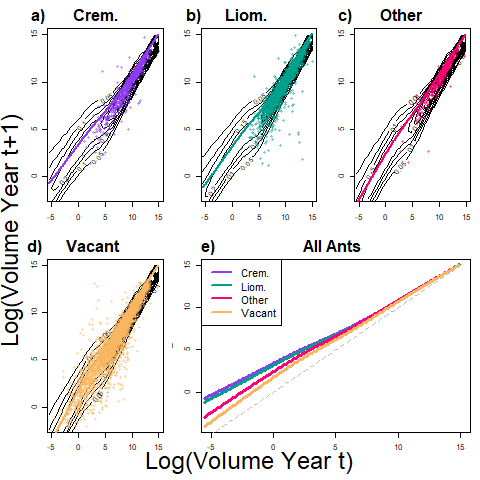
\includegraphics[width = 0.75\linewidth]{Figures/grow_contour_v2.png}
	\caption{The next predicted size of tree cholla based on previous size in relation to ant partner (a, \textit{C. opuntiae}; b, \textit{L. apiculatum}; c, Other; d, Vacant, e, all states combined). Points show observed size transitions, colored lines are the mean next size, and contours show probability density of the skewed normal growth model.  
	Dashed lines indicate extrapolation while solid lines indicate the range of observed data.}
	\label{fig:Grow}
\end{figure}

\begin{figure}[H]
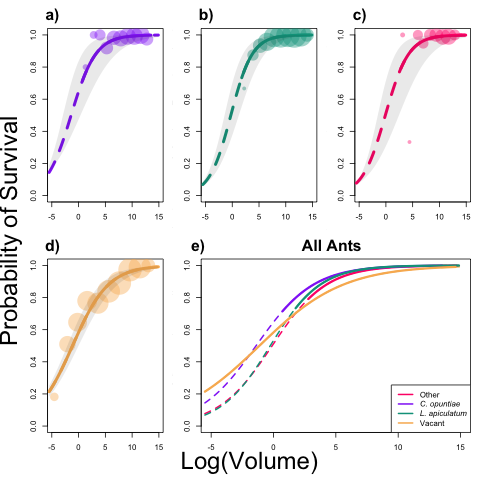
\includegraphics[width=0.75\linewidth]{Figures/survival_plot.png}
\caption{Probability of survival in relation to size and ant partner. Layout as in Fig. \ref{fig:Grow}, except here points show data as binned means, where point size is proportional to number of observations. Grey areas show the 90\% confidence interval for the mean.}
\label{fig:Surv}
\end{figure}

Ant visitation was associated with increased floral viability and ant identity determined the strength of viability benefits.
Mean viability rates spanned 55--81\% (Figure \ref{fig:Viab}).
\textit{L. apiculatum}-tended plants had the highest mean viability rate (86.1\% [95\% credible interval: 77.6--92.4\%]), while there were similar viability rates for vacant (60.0\% [44.3--75.0\%]), Other-tended (60.6\% [43.7--75.5\%]), and \textit{C. opuntiae}-tended plants (57.1\% [40.6--72\%]). 
Furthermore, \textit{C. opuntiae}-tended plants had fewer seeds per fruit (115.0[79.5--165.5] seeds) than vacant (147.2[114.1--189.9] seeds) or \textit{L. apiculatum}-tended plants (142.4[100.7--200.2] seeds), likely due to pollinator interference \citep{Ohm2014}.


\begin{figure}[H]
	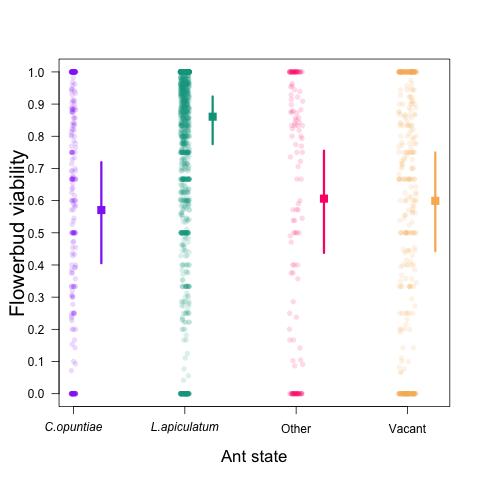
\includegraphics[width=0.95\linewidth]{Figures/Viab_v2.png}
	\caption{Flowerbud viability in relation to ant partner status. Points show observed data (fraction of initiated buds that flower). Points and bars show the means and 95\% credible intervals for each group.}
	\label{fig:Viab}
\end{figure}

%The results of all other vital rates as well as the posterior predictive checks are all included in the Appendix A : Figures S\ref{app:AppA_Seeds_Per_Fruit} -- \ref{app:AppA_Pre_Census_Surv}.

Inter-annual fluctuations in demographic rates (estimated as statistical random effects) were generally positively correlated between ant states, limiting the potential for benefits of diversity through the portfolio effect (Figure \ref{fig:Annual_Ant}). 
However, the degree of correlation depended on the vital rate and pair of ant partners. 
Across vital rates, random effects for cactus growth were the most strongly correlated between ant states (mean pairwise correlation: 0.63) and random effects for survival were the least correlated (mean pairwise correlation: 0.36).  
Certain partner pair / vital rate combinations were effectively independent in their yearly fluctuations (such as survival of \textit{C. opuntiae} and Other-tended plants) while others were almost completely synchronous (such as growth of Vacant and \textit{L. apiculatum}-tended plants). 

\begin{figure}[H]
	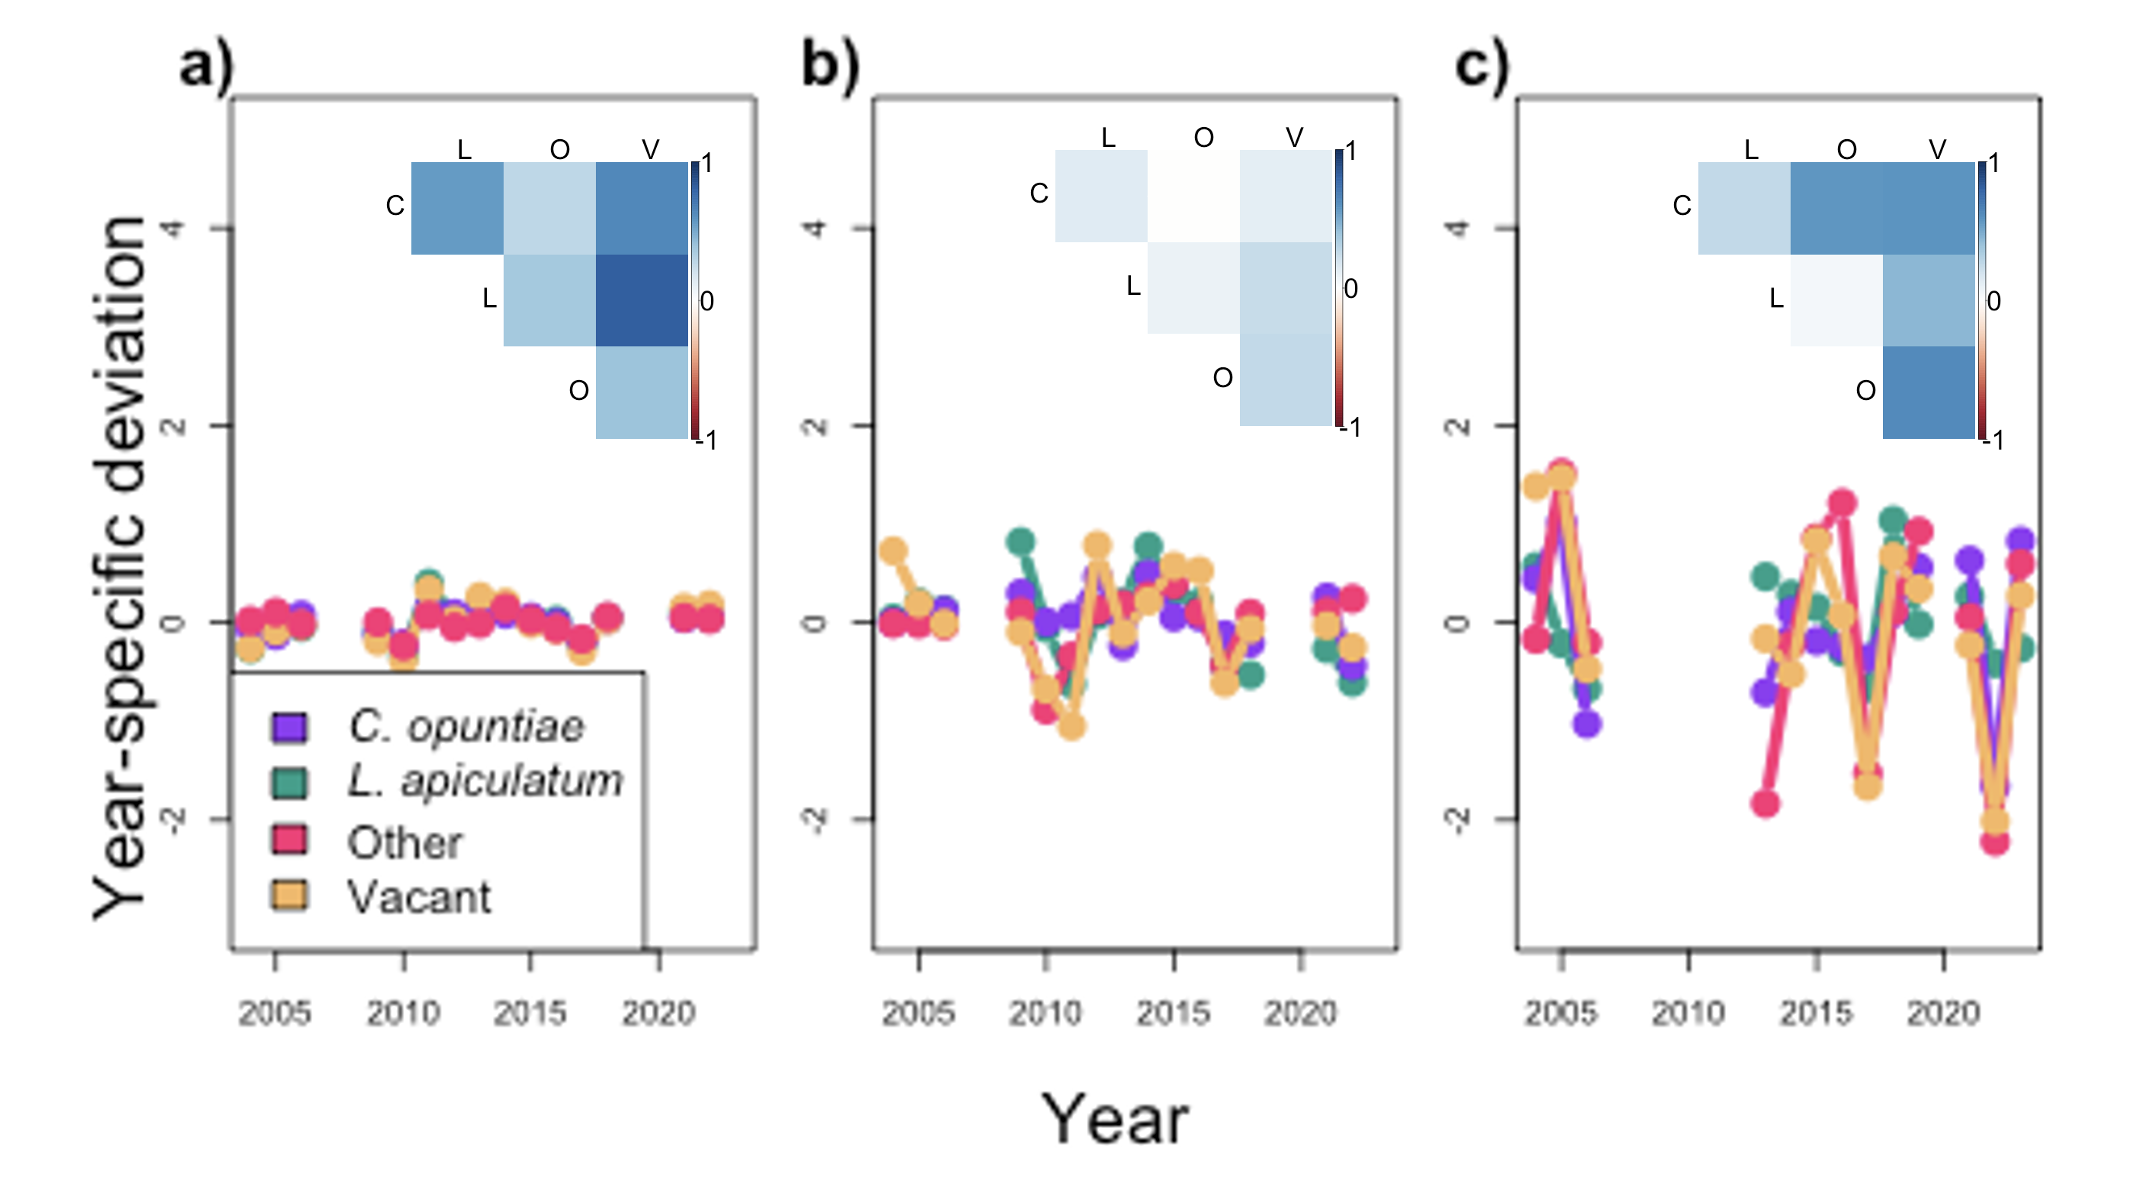
\includegraphics[width=0.75\linewidth]{Figures/ant_RFX.png}
	\caption{Year-specific random effects from statistical models for growth (a), survival (b), and floral viability (c) in relation to ant partner status. Inset panels show correlation coefficients (Pearson's \textit{r}) for each pair of time series. All random effects have mean zero such that positive values indicate better-than-average years and negative values indicate worse-than-average years. Values are missing where there were no data available for that year.}
	\label{fig:Annual_Ant}
\end{figure}

\subsection*{What are the frequency and direction of partner turnover across the plant life cycle?}
A majority (55\%) of plants surveyed in the long-term data experienced at least one ant state transition, with distinct size-dependent and directional patterns (Figure \ref{fig:Ant_Transition}). 
Vacancy was the most likely ant state of small plants ($\leq 10 log(cm^3)$).
Even when small plants were ant-tended at the start of the transition year, they were most likely to transition back to vacancy (Figure \ref{fig:Ant_Transition} b-d). 
The probability of becoming ant-tended increased with size, though it was not equally likely to be tended by any partner.  
For large plants that were initially vacant or tended by \textit{L. apiculatum} or Other ants, \textit{L. apiculatum} was the most likely next partner, suggesting that this species is able to colonize plants that were previously vacant or occupied by Other ants, and effectively retain plants that it previously occupied.  
\textit{C. opuntiae} were also able to retain plants they previously occupied, but not as well as \textit{L. apiculatum}: for plants that began the transition year with \textit{C. opuntiae}, the probability that those plants remain occupied by \textit{C. opuntiae} at the end of the transition year is only slightly greater than the probability of take-over by \textit{L. apiculatum}, while take-over in the other direction was extremely rare. 
It is also notable that transitions away from the initial state of \textit{L. apiculatum} were almost always transitions to vacancy (Figure \ref{fig:Ant_Transition} d), while transitions away from the initial states of \textit{C. opuntiae} and Other  were often transitions to other ants. 
This suggests a competitive hierarchy whereby \textit{L. apiculatum} may abandon low-value plants with little nectar production but is almost never displaced from high-value plants. 

\begin{figure}[H]
	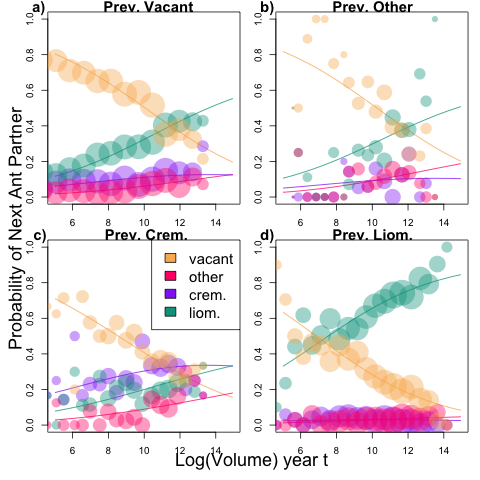
\includegraphics[width=0.95\linewidth]{Figures/transition.png}
	\caption{The probability of ant state based on size and previous ant state. Each panel shows size-dependent probabilities of the next ant state conditional on the previous ant state and size. Solid lines represent predictions of the multinomial statistical model and points show data binned over size intervals, where point size is proportional to the number of observations.}
	\label{fig:Ant_Transition}
\end{figure}

\subsection*{What is the net effect of partner diversity on plant fitness, and what mechanism(s) explain(s) this effect?}
By integrating vital rates, temporal fluctuations, and ant transition dynamics into the stochastic, multi-state IPM we can evaluate the fitness implications of different scenarios of partner identity and diversity (Figure \ref{fig:LambdaMeans}). 
First, there was strong evidence that ant visitation had mutualistic fitness effects on plant partners. 
The lowest mean stochastic fitness was $\lambda^{0}_{S}$, the fitness of the cholla with no partners (Figure \ref{fig:LambdaMeans} a).
Across all 1+ partner scenarios, we found that the $\lambda^{1+}_{S}$ posterior distributions were greater than $\lambda^{0}_{S}$ with nearly 100\% certainty.
This indicates that ant visitation elevates fitness no matter the number of partners.
Furthermore, we found no benefit of partner diversity, with the fitness associated with one, two, or three partners roughly equivalent (Figure \ref{fig:LambdaMeans} a).
The one- and two-partner scenarios were statistically consistent but there was a modest reduction in fitness in the three-partner scenario compared to two partners ($Pr(\Delta\lambda^{2-3}_{S}=0.95)$), consistent with a weak cost of diversity at the highest level.
Patterns of $\lambda_{S}$ in relation to partner richness were generally consistent between scenarios of non-synchronous and synchronous inter-annual fluctuations. 
%The contrasts of $\lambda_{NS}$ posterior distributions of 1 or 2 partner diversity scenarios to $\lambda_{NS}$ posterior distribution of 3 partners show that the overlap ranges from 58\% - 100\%, indicating high similarity between thr full partner diversity scenario and others.
%This is highlighted in Figure \ref{fig:LambdaMeans} panel b.

\begin{figure}
	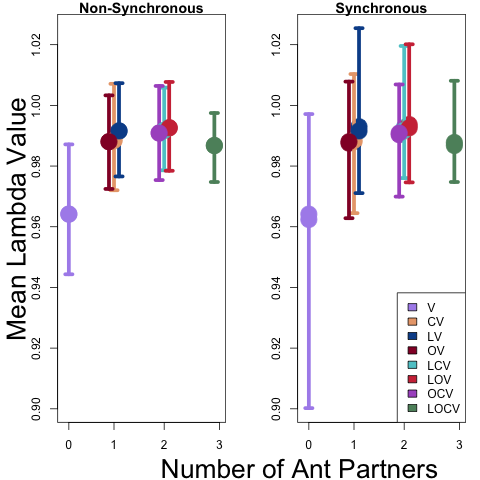
\includegraphics[width=0.91\linewidth]{Figures/Lambdas_Comp_lines.png}
	\caption{Tree cholla stochastic growth rate ($\lambda_{S}$) corresponding to number (a) or number and identity (b-c) of ant partners for synchronous and non-synchronous inter-annual fluctuations. Points and intervals show mean and 95\% credible intervals from the posterior distributions of $\lambda_{S}$. In b-c letters in the legend correspond to ant partners as follows (V = Vacant, C = \textit{C. opuntiae}, L = \textit{L. apiculatum}, O = other).}
	\label{fig:LambdaMeans}
\end{figure}

Partner identity and composition were not strongly consequential for plant fitness (Figure \ref{fig:LambdaMeans} b-c). 
Among the one-partner scenarios, there was no strong evidence for any single best partner species (Figure \ref{fig:LambdaMeans} b). 
While a hypothetical \textit{L. apiculatum}-only population had the highest mean fitness, it was not significantly higher than \textit{C. opuntiae}-  ($Pr(\Delta\lambda^{L-C}_{S}=0.7)$) or Other- ($Pr(\Delta\lambda^{L-O}_{S}=0.69)$) only populations. 
Furthermore, the fitness of \textit{L. apiculatum}-only was consistent with all 2-partner scenarios ($Pr(\Delta\lambda_{S})$ ranged from 0.37 to 0.83).
However, as above, there was evidence for an opportunity cost of diversity wherein fitness of the three-partner scenario was lower than any of the 2-partner scenarios ($Pr(\Delta\lambda_{S})>0.95$). 
The lack of diversity benefits are not driven by the high overall frequency of \textit{L. apiculatum}. 
Using the simulations where all ants had equal frequencies across sizes (further explained in Appendix C), we found the same fitness patterns as described above.
%Equal probability for transitioning into any ant state meant that the numbers of \textit{C. opuntiae} and Other ants were boosted significantly.
%Despite this, the fitness of scenarios including these less frequent ants were not increased meaningfully.

We found no evidence that the portfolio effect generated positive effects of partner diversity, as effects of partner richness and composition were highly consistent between the baseline, non-synchronous model and the model version that synchronized all ant states (Figure \ref{fig:LambdaMeans}).
The effect of all ant partners can be measured as $\lambda^{3}_{S} - \lambda^{0}_{S}$.
We have high confidence that this contrast is positive, and equally so for the synchronous and non-synchronous scenarios (Figure S\ref{fig:Portfolio}).

\section*{Discussion}
% mini abstract paragraph
Mutualisms commonly involve multiple partners but the ecological consequences of partner diversity remain poorly understood. 
Here we show that while alternative partners may be ecologically different, their fitness effects on a shared mutualist can be effectively interchangeable and redundant.
The results of our hierarchical models revealed that different ant partners exhibit different effects on vital rates, with \textit{C. opuntiae}-tended plants experiencing advantages in growth and survival when small, and \textit{L. apiculatum}-tended plants experiencing floral viability advantages. 
These results, alone, would suggest some potential benefits of partner diversity through complementarity.  
Yet, our stochastic, multi-state IPM revealed that all scenarios which included any partners resulted in similarly high cactus fitness, with a statistically significant but quantitatively weak cost of diversity at the highest level. 
Furthermore, evidence from nearly two decades of demographic data failed to support the ``portfolio effect'' hypothesis, whereby benefits of diversity manifest in the context of environmental fluctuations. 
Overall, our results indicate that while ant visitation is strongly consequential, partner composition is much less so, suggesting that the fitness benefits of mutualism from the plant's perspective may be surprisingly resilient to declines in partner diversity. 

% why we see these effects in OUR population
We attribute weak effects of partner identity and diversity to the vital rate sensitivity structure of this population. 
Like other long-lived, iteroparous species \citep{Franco2004}, tree cholla fitness is most sensitive to the growth and survival of established individuals \citep{Miller2009,elderd2016quantifying}, which are virtually guaranteed many years of reproductive opportunities once they reach a size that is protected from mortality. 
Differences between alternative partners were most pronounced either in reproductive rates (floral viability and seed number), which contribute relatively weakly to fitness because a long reproductive lifespan overrides individual reproductive bouts, or in growth and survival at small sizes, where mortality risk is relatively high. 
At larger sizes with low mortality risk, ant-tended plants had consistent growth and survival advantages over vacant plants regardless of partner identity, and that result dominates our integrative measures of fitness; differences between partner species in other vital rates and at other sizes do not register nearly as strongly. 
The weak reduction in fitness at the highest partner diversity level is harder to explain, but suggests some form of missed opportunity cost in a more crowded partner environment. 

Our results broaden the literature on multi-species mutualisms, a majority of which has demonstrated positive effects of partner diversity through complementarity \citep{Yang2024,Hernandez2020,Larimer2014,Afkhami2016,Fehling2022,Gustafson2005,McKeon2012,Palmer2010,Afkhami2021,Stachowicz2005} or portfolio effect \citep{Stevens2024,Thibaut2012,rogers2014,Lazaro2022}. 
For example, working in another sequentially-partnered ant protective mutualism of long-lived plants (\textit{Acacia drepanolobium}), Palmer et al. \citeyear{Palmer2010} showed that synergies between alternative partners elevate plant fitness above what could be expected from the single best partner. 
However, the \textit{Acacia} partner guild includes a ``castrating'' parasite that is uniquely able to boost plant growth by suppressing reproduction. 
We speculate that partners that differ in degree but not type, such as those in our system, may be less likely to synergize. 
Fewer studies have shown costs of mutualist diversity. 
Bruna et al. \citeyear{Bruna2014} showed that ant diversity can depress fitness of the sequentially-partnered ant-plant \textit{Maieta guianensis} due to reduced interactions with the better defender. 
Costs of diversity have also been documented in systems in which multiple partners interact simultaneously with a shared mutualist, likely due to interference via the host resource budget \citep{Keller2018} or negative higher-order interactions \citep{Barrett2015}. 
One previous study (in a different ant-cactus system) showed neutral effects of partner diversity, but this study also showed that ant visitation was itself neutral, with no detectable effects on plant fitness \citep{Ford2015}. 
To our knowledge, ours is the first study documenting a strong, positive fitness effect of mutualism, regardless of mutualist identity or guild composition. 
As this field grows, particularly with studies that integrate multiple vital rates across the life cycle, we will be better positioned to understand whether positive, neutral, or negative effects of partner diversity predominate, and the conditions under which each might be more likely. 

% Portfolio Effect
When partners exhibit different reactions to varying environments, interacting with a diverse portfolio of partners can lead to more consistent benefits across time \citep{Batstone2018}.
Our work explicitly incorporated temporal environmental stochasticity, yet we find no evidence for the portfolio effect as a mechanism of diversity benefits. 
In ant-plant defensive mutualisms, any portfolio effect would emerge from fluctuations in the community of herbivores, and ant-specific responses to each herbivore species. 
Instead, we found that inter-annual fluctuations in vital rates were largely synchronized across plants in different ant states, suggesting other drivers of inter-annual variation that are shared across the population -- notably, weather -- override any fluctuations in herbivore composition and ant-herbivore interactions. 
Dallas et al. \citeyear{dallas2022temporal} found that while the portfolio effect was easy to show in theoretical models, it is infrequently detected in empirical data across many systems. 
This indicates that the portfolio effect may be difficult to detect, disguised by different mechanisms, or uncommon in nature. 

% Value of Long-term data
This study highlights the value of long-term data in investigating species interactions. 
Previously studies have analyzed how partner identity and partner turnover impact focal mutualist fitness \citep{Fonseca2003, Dejean2008, Noe1994, Barrett2015, Bruna2014, Trojelsgaard2015}.
Separate studies have analyzed how inter-annual variability impacts focal mutualists \citep{Alonso1998, Alarcon2008, Ollerton2006, Horvitz1990, Lazaro2022}.
The long term data set we used gave us the ability to consider, for the first time, the combined effects of partner identity, partner turnover, and temporal stochasticity. 
By piecing together complete life cycle information from long-term data, we gain a more nuanced understanding of the fitness consequences of ant visitation. 
For example, our previous study that focused only on reproductive vital rates suggested that \textit{C. opuntiae} has overall parasitic fitness effects because activity of this species within tree cholla flowers can deter pollinators and reduce seed set \citep{Ohm2014}. 
Yet, the more complete analysis presented here, which accounts for reduced seed set alongside other demographic advantages in higher-sensitivity vital rates, indicates that this species is clearly a mutualist. 

% Limitations
As with any study, there are limitations to consider when interpreting our results.
First, we used observational data to infer ant effects on plant demography. 
However, we have previously conducted experimental manipulations which revealed that ant presence has causal effects on plant demographic rates through anti-herbivore defense \citep{Miller2007,Ohm2014}.
The combination of long-term observational data backed up by experimental results gives us greater confidence in our causal interpretations. 
Second, we have not explicitly incorporated ant-herbivore interactions, even as these are the primary pathway through which ants influence plant demography. 
Surveys of herbivore damage from our long-term data are consistent with protective benefits of ant visitation \tom{(Figure \ref{app:herb})}{Note that this is referencing Figure 2, which is not correct.}, and more explicit inclusion of plant-herbivore-defender interactions could be a valuable future direction. 
Third, the rarity of several ant partner species imposed a practical constraint on assessing effects of partner diversity, since we needed to combine these into an ``Other'' category that might mask important differences. 
As more long-term data accumulate, we may gain more information with which to further unpack this group of species. 

% tie back paragraph.
\paragraph{Conclusion}
This study highlights that while partners within a mutualistic guild can be ecologically different, they may still be interchangeable in their net effects on fitness of a shared mutualist based on where their effects occur in the life cycle. 
Contrary to much of the literature on multi-species mutualisms, we find that while ant partners are beneficial, partner diversity has no measurable benefit to their shared mutualist and may even be somewhat costly. 
As studies accumulate across different types of multi-partner mutualisms, particularly those spanning simultaneous/sequential partnerships and leveraging demographic data from the complete life cycle, our field will be better poised to understand whether, how, and under what conditions mutualist diversity is neutral, costly, or beneficial.


\section*{Acknowledgments}
Financial support for this work came from the Sevilleta Long-Term Ecological Research Program (NSF DEB awards 1655499 and 1748133).
We acknowledge the many students and technicians who have helped collect annual census data for this project, including M. Donald, J. Fowler, M. Saucedo, K. Dickens, T. Jordan-Millet, J. Moutouama, C. Oxley, K. Schraeder, B. Scherick, A. Sears, M. Tucker, and J. Xiong. 
J. Moutouama, A. Bradley, B. Scherick, A. Gough, J. Martin, and V. Rudolf provided helpful feedback on the manuscript. 


%%%%%%%%%%%%%%%%%%%%%
% Statement of Authorship
%%%%%%%%%%%%%%%%%%%%%
% This section should also be commented out while your MS is undergoing
% double-blind review. The specifics should of course be adapted to
% your paper, but the paragraph below gives some hints of possible
% contributions.

\section*{Data and Code Availability}
Most of the data that support the findings of this study (through 2019) are openly available as a \href{https://portal.edirepository.org/nis/mapbrowse?packageid=knb-lter-sev.323.1}{data package} \citep{DataCholla} on the Environmental Data Initiative website, package id: knb-lter-sev.323.1.
An updated data package, including recent years, is presently under review and we expect will be available in early 2025. 
For now, all of our data and code are available in our public github repo: \url{https://github.com/acampbell110/ant_cactus_demography}.


\renewcommand{\theequation}{A\arabic{equation}}
% redefine the command that creates the equation number.
\renewcommand{\thetable}{A\arabic{table}}
\setcounter{equation}{0}  % reset counter 
\setcounter{figure}{0}
\setcounter{table}{0}

%%%%%%%%%%%%%%%%%%%%%
% Bibliography
%%%%%%%%%%%%%%%%%%%%%
% You can either type your references following the examples below, or
% compile your BiBTeX database and paste the contents of your .bbl file
% here. The amnatnat.bst style file should work for this---but please
% let us know if you run into any hitches with it!
%
% If you upload a .bib file with your submission, please upload the .bbl
% file as well; this will be required for typesetting.
%
% The list below includes sample journal articles, book chapters, and
% Dryad references.
\bibliographystyle{apalike}
\bibliography{References.bib}


\newpage{}


\appendix
\label{appendix}
\section*{Appendix A: Additional Methods and Parameters} \label{appendix:A}
In addition to the models described in the body of the paper, we fit several other models using data from previous studies.
These models are described below.

\paragraph{Seeds Per Fruit}
With data from \cite{Miller2006}, we fit a model for the number of seeds produced by every fruit on a cholla ($\kappa(a')$) in year $t+1$ based on the ant partner $a'$ in year $t+1$.
We fit this model to seed data $y^{\kappa}$ using a Negative Binomial distribution and the log link function: 
$$y^{\kappa} \sim  Negative Binomial(\hat{\kappa},\hat{\phi})$$
$$\hat{\phi} = \beta_{0}^{\phi}$$
The data used for this model did not include data on ants in the ``other" category, so we used the data from vacant plants to parameterize seeds per flower for plants with ``other" ants in the IPM.

We found that vacant plants produced the most mean seeds (147.2 per fruit), followed by \textit{L. apiculatum} tended plants (142.4 per fruit), and finally, \textit{C. opuntiae} tended plants (115.0 per fruit).


\paragraph{Recruit Size Distribution}
We fit this model to recruit size data $y^{\eta}$ using a Normal distribution with the identity link function: 
$$y^{\eta} ~\sim N(\hat{\eta},\hat{\sigma})$$
where $\hat{\sigma}$ is estimated with a non-informative prior. 

We found that the mean size of recruits is $log(-2.097) m^3$ with an interquartile range from $log(-2.173) m^3$ to $log(-1.712) m^3$.



\paragraph{Germination}
With germination data \cite{Miller2007}, we fit two models for the probability of germinating from the first year seedbank ($\gamma_1$) or the second year seedbank ($\gamma_2$) in year $t+1$, with no fixed or random effects.
These models were fit to germination data $y^{\gamma_1}, y^{\gamma_2}$  using the binomial distribution with logit link functions:
$$y^{\gamma_1} \sim Binomial(\hat{\gamma_1})$$
$$y^{\gamma_2} \sim Binomial(\hat{\gamma_2})$$

We found that the mean germination rates for seeds in the seedbank for one year  is 0\%, with an interquartile range of 0\% and 1\%.
We found that the mean germination rates for seeds in the seedbank for a second year is 0\%, with an interquartile range of 0\% to 0.4\%.
Seeds are more likely to germinate in their first year in the seedbank, but most seeds will never germinate. 

\paragraph{Pre-Census Survival}
With recruit census data \cite{Miller2006}, we fit a model for the probability of a seedling (which germinates in early Fall) surviving to when we census in May ($\delta$) of year $t+1$ (accounting for missed mortality events), with fixed effects of the previous size $x$ and random effects of the transect $m$.
We fit this model to pre-census survival data $y^{\delta}$ using a Bernoulli distribution with a logit link function: 
$$y^{\delta} ~ Bern(\hat{\delta})$$
where $m \sim N(0, \sigma_{transect}^2)$ is the random effect of transect where the recruited individual was analyzed for survival.

We found that plants have a 16.2\% probability of surviving from germination to the next census.
Our model estimated this very well, expecting a 16.3\% probability.


\paragraph{Portfolio Effect}
We compared the effects of partner diversity (estimated as $\lambda_S^4 - \lambda_S^0$) for the synchronized and non-synchronized models.
We determined that non-synchronous effects of ant partners are greater than synchronous effects of ant partners only 50\% of the time.
This means there is no evidence of portfolio effect in this system.


\begin{figure}[H]
	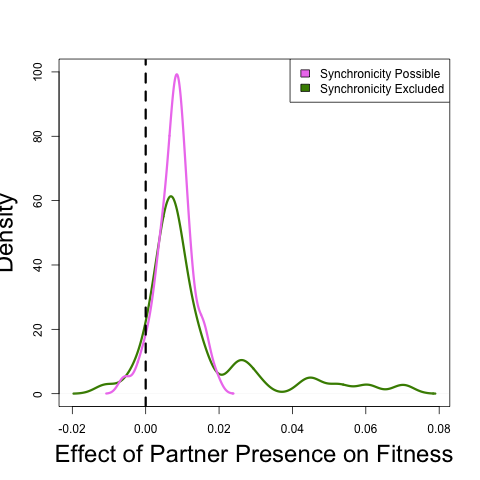
\includegraphics[width=\linewidth]{Figures/portfolio_effect.png}
	\caption{The distributions of $\lambda_{S}^4-\lambda_{S}^0$ for the non-synchronous and synchronous models are shown in pink and green respectively. The vertical dashed line shows where the effect of partners on the fitness of the cholla is 0 (to the left the partners have a negative effect, to the right the partners are beneficial).}
	\label{fig:Portfolio}
\end{figure}

\section*{Appendix B: Observed Herbivory Data} \label{appendix:B}
Herbivory is an important driver in this population and shapes the range and demography of cholla.
Herbivore presence has been shown to negatively impact growth and fecundity of cholla populations \citep{Miller2009}.
Ant visitors are believed to offer defensive benefits to the plants they tend in this system, leading to the hypothesis that ant presence would be correlated with reduced herbivory.
Therefore, herbivore protection is the likely driver behind the increased survival, growth, and reproductive rates of tended plants. 
Fluctuations in herbivore communities across time would also lead to potentially important fluctuations in ant visitor responses and therefore cholla demographic responses.

Here we conduct  an analyses of herbivory levels on plants with different ant visitors and contrast them to herbivory levels on plants with no visitors.
Evidence that herbivory is decreased for tended plants further strengthens the results presented in this paper that ant presence is beneficial on a demographic level for cholla.

Herbivory data was collected during censuses any time herbivores were identified on a plant. 
This involved noting the type and quantity of herbivores observed. 
This data has been taken consistently since 2017, so the analysis below considers 6 years of data.
We considered only plants which were reproducing, since prior work shows that flowering significantly elevates herbivore pressure \citep{Miller2006}.
The proportion of reproducing plants that experienced herbivory was calculated for each ant state separately.
Analysis showed that ant presence is correlated with lower herbivore visitation.
40\% of vacant cacti experienced herbivory.
Plants tended by Other ants experienced similar, though lower, levels of herbivory on reproducing plants, with herbivores detected on 37.5\% of plants.
Herbivores were detected on 25\% of plants tended by \textit{C. opuntiae} ants and on 11\% of plants tended by \textit{L. apiculatum} ants.
These results indicate that ant presence is correlated with lower levels of herbivory and that partner identity has an impact on the level of herbivory.
They also indicate that the partner correlated with the lowest levels of herbivory is \textit{L. apiculatum} ants.
These findings are consistent with literature findings which show that \textit{L. apiculatum} ants are the most aggressive (therefore the most effective against herbivores), but differ from previous findings that \textit{C. opuntiae} may not offer defensive benefits \citep{Miller2007}.


\begin{figure}[H]
	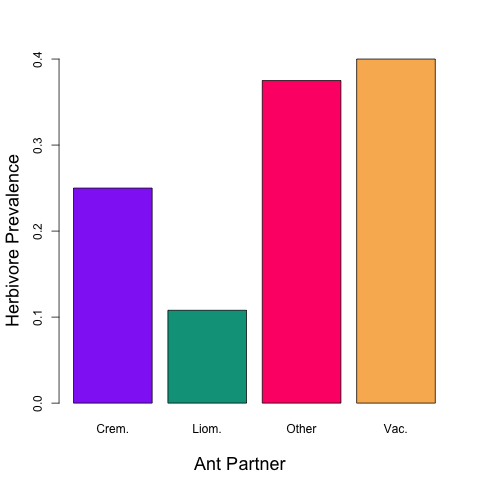
\includegraphics[width=0.7\linewidth]{Figures/herb_all.png}
	\caption{The proportion of reproducing plants which are visited by herbivores. Each bar represents the subset of the cacti population in a different ant state.  }
	\label{app:herb}
\end{figure}



\section*{Appendix C: Alternative Ant Transition Simulations}\label{appendix:C}
In addition to the competitive exclusion model defined and analyzed in the body of the paper, we simulated results from several other potential models. 
We chose to include competitive exclusion as our primary results in the paper because we believe it to be the most biologically realistic.
However, in building and testing of alternative models we found that the method of ants occupying plants significantly impacts the fitness of the population. 
We tested two alternative transition models, one called the frequency based model and one called the equal likelihood model. 

\paragraph{Frequency Based Model}
The first alternative hypothesis we tested was what we called the frequncy based model.
In this model rather than the proportion of vacant cacti being maintained, the proportion of cacti occupied by each species is maintained and when one is removed it is replaced with vacancy.
This version of the model assumes that the frequency of each ant we see is reflective of the real frequency of populations rather than some other mechanism.
With this model we found very clear evidence of Sampling Effect in the system. 
When only  \textit{C. opuntiae}, Other ants, or both ants are present, there is very little difference in the fitness of the cacti from when no partners are present. 
Only when \textit{L. apiculatum} ants are present do we see an increase in the fitness of the focal mutualist (Figure \ref{app:FreqLambdaMeans}a).
In this simulation, the more partners that are present the higher the fitness of the focal mutualist is, confirming that partner diversity would be beneficial through sampling effect if this transition model were correct.  (Figure \ref{app:FreqLambdaMeans}b).

\begin{figure}
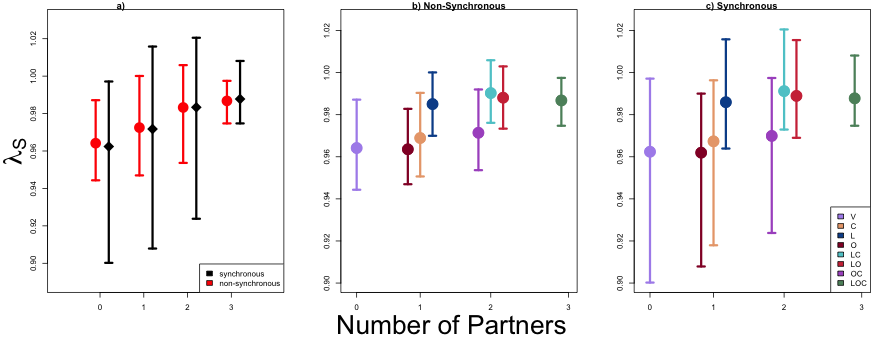
\includegraphics[width=0.91\linewidth]{Figures/Lambdas_Freq_lines.png}
	\caption{Panel a) the mean estimated $\lambda_{NS}$ and $\lambda_{S}$ for different numbers of partners (0-3) for the synchronous IPM (black circle) and the non-synchronous IPM (red diamond). The lines show the posterior distribution spread of the estimated $\lambda$ values. Panels b-c) the mean estimated $\lambda_{NS}$ and $\lambda_{S}$ respectively, for each simulated combination of ant partner as the filled in circles. The lines show the posterior distribution spread of estimated $\lambda$ values. The letters in the legend correspond to what ant partners are present (V = Vacant, C = \textit{C. opuntiae}, L = \textit{L. apiculatum}, O = other).}
\label{app:FreqLambdaMeans}
\end{figure}

\paragraph{Equal Likelihood Model}
The second alternative hypothesis we tested was what we called the equal likelihood model.
In this model we preserved the observed pattern of size-dependent vacancy/occupancy, but occupancy was manipulated to be equally likely for all partner identities. 
This was designed to remove the effect overwhelming numbers of \textit{L. apiculatum} ants may have. 
Despite very different proportions, we found very similar outcomes to the competitive exclusion model analyzed in the paper. 
All ants are beneficial, but having more than one is not necessarily any better than having an individual species as a partner (Figure \ref{app:EqualLambdaMeans}b).
Partner presence is beneficial, but neither identity nor number of partners appears to be important (Figure \ref{app:EqualLambdaMeans}a).

\begin{figure}
\includegraphics[width=0.91\linewidth]{Figures/Lambdas_equal_lines.png}
	\caption{Panel a) the mean estimated $\lambda_{NS}$ and $\lambda_{S}$ for different numbers of partners (0-3) for the synchronous IPM (black circle) and the non-synchronous IPM (red diamond). The lines show the posterior distribution spread of the estimated $\lambda$ values. Panels b-c) the mean estimated $\lambda_{NS}$ and $\lambda_{S}$ respectively, for each simulated combination of ant partner as the filled in circles. The lines show the posterior distribution spread of estimated $\lambda$ values. The letters in the legend correspond to what ant partners are present (V = Vacant, C = \textit{C. opuntiae}, L = \textit{L. apiculatum}, O = other).}
\label{app:EqualLambdaMeans}
\end{figure}


\section*{}\label{appendix:D}
Below are the results reported of all statistical models not described in the main body of the text. 

%% Reproduction Model
\paragraph{Reproduction Model}
\tom{The probability of a plant reproducing in a given year is highly size dependent. 
The mean probability of reproducing remains at about 0\% until the plant reaches a medium size, after which the mean probability of reproducing increases steadily before reaching about 100\% at large sizes. }{What about the flowerbud model? I think there is value is showing the data and model fit (here in the appendix) for both Pf(flowering) and \# flowerbuds vs size.}


%% Seeds Produced
\paragraph{Seeds Per Flower Model}
\tom{Each viable flower on a plant produces between 97 and 257 seeds.}{You had a figure showing mean seeds per fruit by ant group. I think you should keep that figure here.}
This number is affected by the ant partner present, as shown in previous work \citep{Ohm2014}. 
\textit{C. opuntiae} tended plants produce a mean of 115 seeds per flower. 
\textit{L. apiculatum} tended plants produce a mean of 143 seeds per flower.
Vacant plants produce a mean of 148 seeds per flower. 
Comparison between posterior distributions revealed that \textit{C. opuntiae} tended plants produced fewer seeds per flower than \textit{L. apiculatum} tended plants and vacant plants 80\% and 87\% of the time.
Vacant plants produced more seeds per flower than \textit{L. apiculatum} tended plants only 57\% of the time.
\tom{We are confident that \textit{C. opuntiae} tended plants produce the fewest seeds per flowers.}{Confident how? What is this based on?}

%% Precensus Survival\
	\paragraph{Pre-census Survival Model}
	Pre-census seed survival rates fall between 0\% and 95\% with the mean pre-census seed survival at 18\%.
	
	%% Germination
	\paragraph{Germination Model}
	\tom{Seeds have a significantly higher probability of germinating in year one than in year two.}{Not sure why you say significantly higher. The posteriors you describe in the next sentence are completely overlapping.}
	Seeds in year one experience germination rates between 50\% and 100\% with a mean of 62\% germination.
	Seeds in year two experience germination rates between 50\% and 98\% with a mean of 58\% germination.
	
	
	%% Recruit size distribution
	New recruits are expected to be between the sizes of 0.11 $cm^3$ and 0.38 $cm^3$ with a mean size of 0.20 $cm^3$.



\end{document}
